% \documentclass[12pt]{report}
\documentclass[11pt,table,xcdraw]{report}

% Fonts
% Greek font
% \usepackage[T1]{fontenc} %% LGR encoding is needed for loading the package gfsneohellenic
% \usepackage[default]{gfsneohellenic}

% Sans serif font
% \usepackage[T1]{fontenc}
% \usepackage{sansmathfonts}
% \renewcommand*\familydefault{\sfdefault} %% Only if the base font of the document is to be sans serif
% \usepackage{lmodern}
% \usepackage{fix-cm}

% TeX Gyre Pagella
\usepackage[T1]{fontenc}
\usepackage{tgpagella}
\usepackage[scaled]{beramono}
% \usepackage{palatino}
% \renewcommand*\familydefault{\sfdefault} %% Only if the base font of the document is to be sans serif
\usepackage{fix-cm}

% Reduce space before chapter title
\usepackage{titlesec}
\titleformat{\chapter}[display]
{\normalfont\huge\bfseries}{\chaptertitlename\ \thechapter}{20pt}{\Huge}
\titlespacing*{\chapter}{0pt}{0pt}{20pt}

% Packages
\usepackage{graphicx}
\usepackage{float}
\usepackage{mathalpha}
\usepackage{amsmath}
\usepackage{amsfonts}
\usepackage{amssymb}
\usepackage{enumitem}
\usepackage{hyperref}
\usepackage{multicol}
\usepackage[super]{nth}
\usepackage{subcaption}
\usepackage[export]{adjustbox}
\usepackage{pdfpages}

% TABLES
\usepackage{xcolor}
\usepackage[normalem]{ulem}
\useunder{\uline}{\ul}{}
\definecolor{llgray}{gray}{0.98}

% Listing in Lisp
\usepackage{listings}
\lstset{
    numbers=left,
    numberstyle=\tiny,
    numbersep=9pt,
    language=Lisp,
    % stringstyle=\ttfamily\small,
    stringstyle=\ttfamily\footnotesize,
    basicstyle=\ttfamily\footnotesize,
    % basicstyle=\ttfamily\scriptsize,
    showstringspaces=false,
    breaklines=true,
    frame=single,
    keywordstyle=\color{purple},
    commentstyle=\color{darkgray},
    backgroundcolor=\color{llgray},
    morekeywords = {gil, om, for, if, setq}
}
% Captions package
\usepackage[hypcap=false]{caption}
\DeclareCaptionType{trans}[Transcription][List of transcriptions]
% Bibliography package
\usepackage[
    backend=biber,
    sorting=none
    % style=authoryear-icomp
]{biblatex}

% Others
\newenvironment{Figure}
  {\par\medskip\noindent\minipage{\linewidth}}
  {\endminipage\par\medskip}

% External files
% \usepackage{xr}
% \externaldocument{Sections/sct_1SP}

% New commands
% TODO counter
\newcounter{todocount}
\newcounter{todosecc}
\newcounter{todoimac}
\setcounter{todocount}{0}
\setcounter{todosecc}{0}
\setcounter{todoimac}{0}
\newcommand{\todo}{\stepcounter{todocount}\textbf{\textcolor{magenta}{TODO \arabic{todocount} }}}
\newcommand{\todosec}{\stepcounter{todosecc}\textbf{\textcolor{blue}{TODO-sec \arabic{todosecc} }}}
\newcommand{\todoimage}{\stepcounter{todoimac}\textbf{\textcolor{red}{TODO-fig \arabic{todoimac} }}}
% shortcut for cantus firmus in italic font
\newcommand{\cf}{\textit{cantus firmus }}
\newcommand{\cfdot}{\textit{cantus firmus. }}
\newcommand{\cfcomma}{\textit{cantus firmus, }}
% shortcut for species
\newcommand{\species}[1]{\nth{#1} species}
% shortcut for B in mathcal
\newcommand{\B}{\mathcal{B}}
% shortcut for N in mathcal
\newcommand{\N}{\mathcal{N}}
% shortcut for R in mathcal
\newcommand{\R}{\mathcal{R}}
% \newcommand{\R}{R}
% shortcut for C in mathcal
\newcommand{\C}{\mathcal{C}}
% shortcut for I in mathcal
\newcommand{\I}{\mathcal{I}}
% shortcut for Lisp ID
\newcommand{\lid}[1]{$\lambda$ID = \texttt{#1}}
% shortcut for default value
\newcommand{\df}[1]{\qquad \textit{DFLT: <#1>}}
\newcommand{\dft}[1]{\textit{DFLT: <#1>}}
\newcommand{\dfts}[1]{\textit{<#1>}}
% shortcut for forall values
\newcommand{\forj}{\forall j \in [0, m-1)}
\newcommand{\forn}{\forall i \in \B, \forall j \in [0, m)}
\newcommand{\fornm}{\forall i \in \B, \forall j \in [0, m-1)}
\newcommand{\fornmm}{\forall i \in \B, \forall j \in [0, m-2)}
\newcommand{\forp}{\forall \rho \in positions(m)}
\newcommand{\forpm}{\forall \rho \in positions(m-1)}
\newcommand{\forpmm}{\forall \rho \in positions(m-2)}
% size used for the height of figures
\newcommand{\fhs}{1.1in}
\newcommand{\fh}{1.2in}
\newcommand{\fhl}{1.3in}

% auto cite from bib
\DeclareCiteCommand{\citea}
{\boolfalse{citetracker}\boolfalse{pagetracker}\usebibmacro{prenote}}
{\href{\thefield{url}}{here}}
{\multicitedelim}
{\usebibmacro{postnote}}
% add "Score available here." sending to url + reference beside
\newcommand{\listen}[1]{Score available \citea{#1} \parencite{#1}}
% add "Listen here." sending to url + reference beside
\newcommand{\listenyt}[1]{and listen \href{#1}{here} \parencite{EvalYT}.}

% Load Bibliography
\addbibresource{Bibliography/cite.bib}

\title{Formalizing Fux's Theory of Musical Counterpoint Using Constraint Programming}
\author{Thibault Wafflard}
\date{June 2023}

% Document settings
% \usepackage[margin=1.3in]{geometry}
\usepackage{geometry}
\geometry{
    a4paper,
    % total={170mm,257mm},
    left=1.3in,
    right=1.3in,
    top=1in,
    bottom=1in,
}

\begin{document}
%\pagenumbering{roman}
% \maketitle
%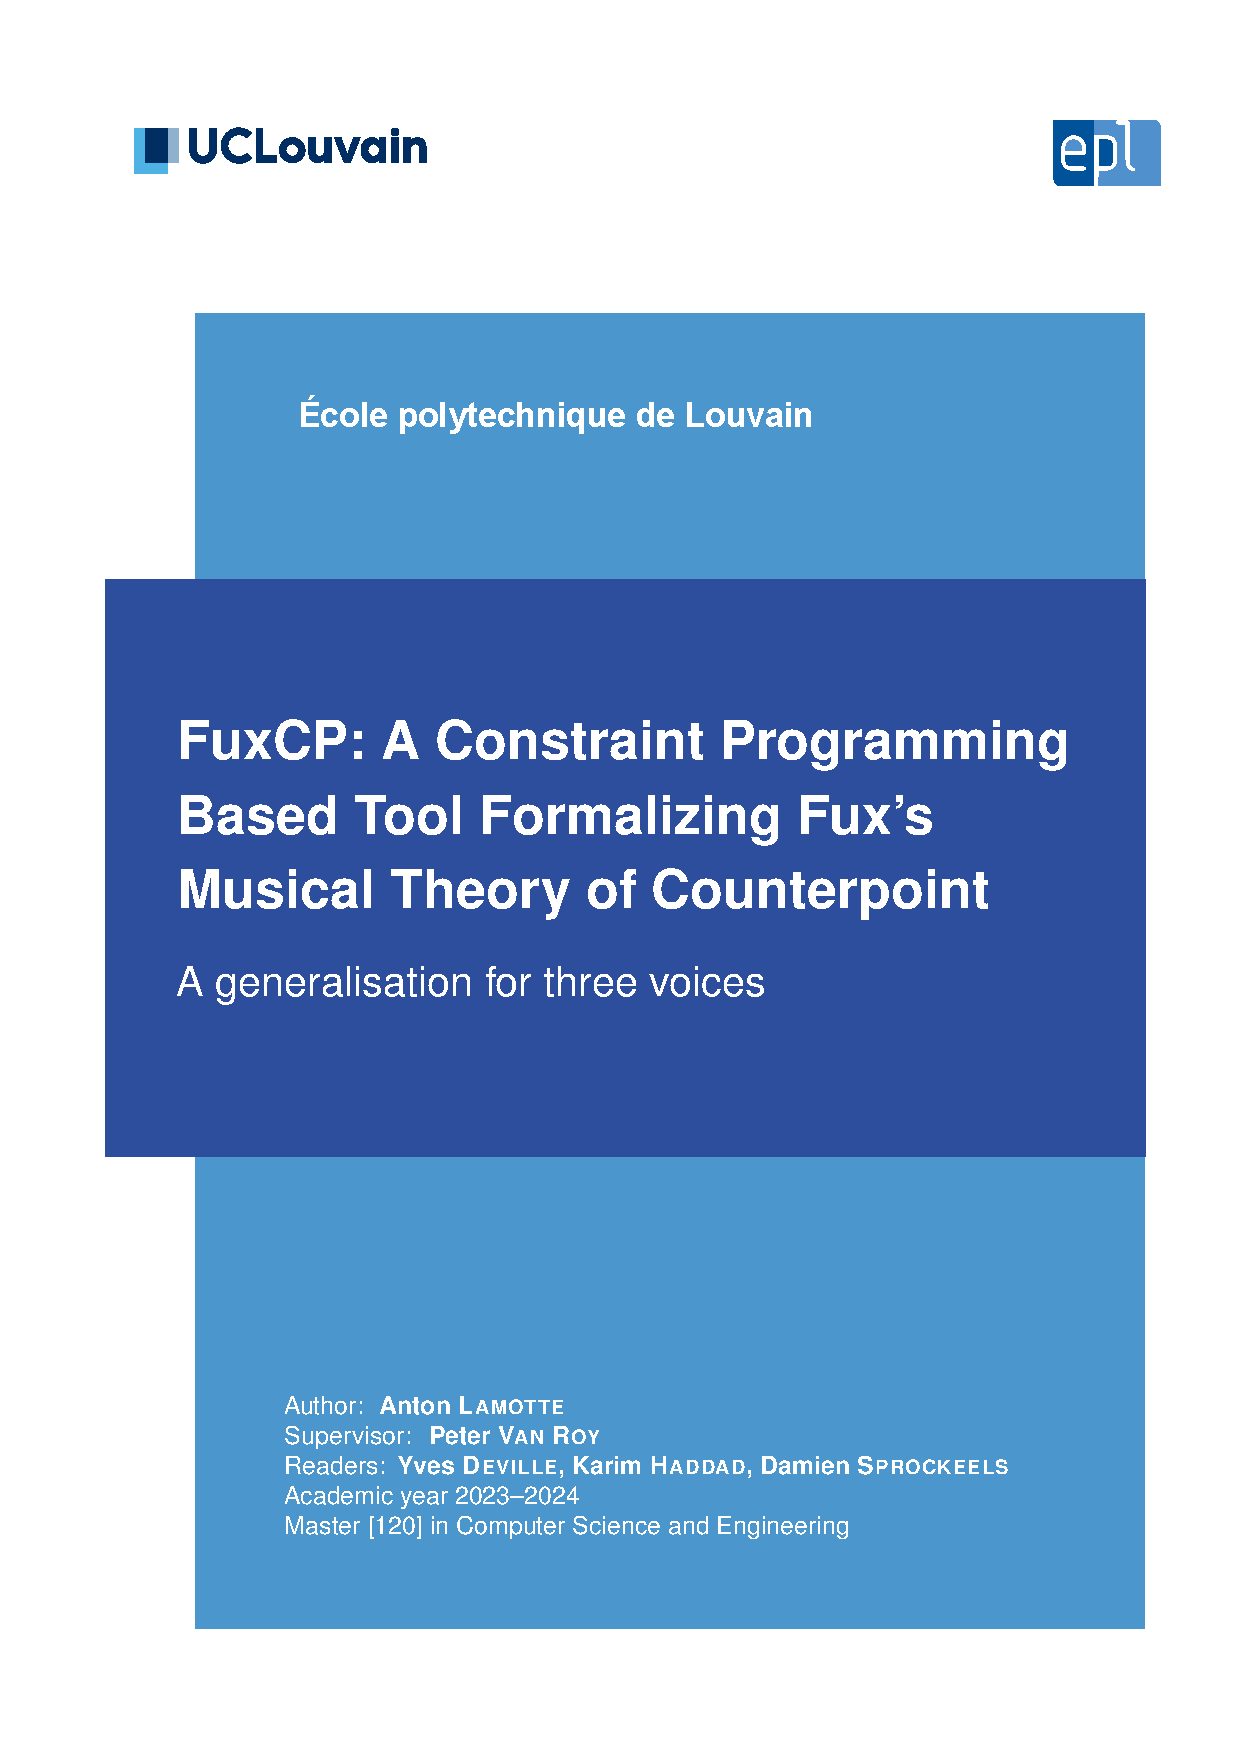
\includepdf[pages=1]{FrontPage.pdf}
%\null
%\thispagestyle{empty}
%\addtocounter{page}{-1}
%\newpage
%\newgeometry{left=1.65in,right=1.65in,top=2in,bottom=2in}
%\begin{abstract}
%    \large{
%        This master's thesis presents FuxCP, a tool for computer-aided contrapuntal composition. The objective is to assist composers without programming skills by automating repetitive and time-consuming tasks. The tool is based on constraint programming with Gecode and formalizes musical rules as constraints. Thanks to this approach, the tool provides transparency and control over the generated solutions, allowing composers to shape their desired music. This thesis focuses on formalizing the rules of two-voice counterpoint from Fux's \textit{Gradus ad Parnassum}. The research highlights the advantages of constraint programming over other approaches, as it allows the tool to "understand" the generated music. The thesis covers the formalization of counterpoint species-specific rules as mathematical constraints, the evaluation of the tool compared to Fux, and suggestions for future development. The conclusion emphasizes the importance of a comprehensive set of rules for formalization, the need for additional constraints on melodic development, and the potential for more expert solvers in other musical genres. The findings indicate the potential of constraint programming in enhancing computer-aided composition across various musical styles.
%    }
%\end{abstract}

%\chapter*{Acknowledgements}
%\paragraph{Thanks to Peter Van Roy}, my supervisor, for giving me the opportunity to write this thesis combining two of my passions: computer science and music.

%\paragraph{Thanks to Damien Sprockeels} for his pragmatic feedback, his devotion to the project, and his great contribution to computer music.

%\paragraph{Thanks to Karim Haddad} from IRCAM for proposing the \textit{Gradus ad Parnassum} as a reference book.

%\paragraph{Thanks to Yves Deville} for reading this thesis.

%\paragraph{Thanks to UCLouvain} for allowing me to finish my studies on such an instructive project.

%\paragraph{Thanks to Justine Nagant} for supporting me throughout this long ordeal.

%\paragraph{It is thanks to} the energy and time of all these people that this thesis exceeded my expectations.
%\restoregeometry

%\tableofcontents
E2.2W means "Equation 2.2 from T. Wafflard's thesis".

S1.3W means "Section 1.3 from T. Wafflard's thesis".

%\addcontentsline{toc}{chapter}{Bibliography}
%\printbibliography

\appendix

% \bibliographystyle{plain}
% \bibliography{Bibliography/cite}

%
\includepdf[pages=1]{BackPage.pdf}
\end{document}